\documentclass[11pt, a4paper]{article}
\newcommand{\HomeworkHeader}{L00\_02}
% Shared LaTeX preamble for homework/*/main.tex

% --- Base layout ---
\usepackage[a4paper, top=2.5cm, bottom=2.5cm, left=2cm, right=2cm]{geometry}
\usepackage{fontspec}
\usepackage{xeCJK} % CJK fallback to avoid missing glyphs in Latin fonts
\usepackage{amsmath, amssymb, amsthm}
\usepackage{mathtools}
\usepackage{fancyhdr}
\usepackage{lastpage}
\usepackage[svgnames]{xcolor}
\usepackage{tikz}
\usetikzlibrary{automata, positioning, arrows.meta, bending, backgrounds}
\usepackage{pgfplots}
\pgfplotsset{compat=1.18}
\usepackage[most]{tcolorbox}
\usepackage{enumitem}

% --- Languages & fonts ---
\usepackage[english]{babel}
\babelprovide[import, main]{chinese}

\babelfont{rm}[UprightFont=*, BoldFont=* Bold, ItalicFont=* Italic, Scale=1.05]{Linux Libertine O}
\babelfont{sf}[UprightFont=*, BoldFont=* Bold, Scale=1.05]{Linux Biolinum O}
\babelfont[chinese]{rm}[
    UprightFont=*-Regular,
    BoldFont=*-Bold,
    ItalicFont=*-Regular,
    BoldItalicFont=*-Bold
]{Noto Serif CJK SC}
\babelfont[chinese]{sf}[
    UprightFont=*-Regular,
    BoldFont=*-Bold
]{Noto Sans CJK SC}
\babelfont{tt}{Noto Sans Mono}
\babelfont[chinese]{tt}{Noto Sans Mono CJK SC}

% xeCJK font setup (kept consistent with babelfont)
\setCJKmainfont{Noto Serif CJK SC}
\setCJKsansfont{Noto Sans CJK SC}
\setCJKmonofont{Noto Sans Mono CJK SC}

% --- Colors ---
\definecolor{primaryColor}{RGB}{46, 52, 64}
\definecolor{accentColor}{RGB}{94, 129, 172}
\definecolor{boxFill}{RGB}{236, 240, 241}
\definecolor{solLine}{RGB}{163, 190, 140}
\definecolor{expandColor}{RGB}{191, 97, 106}

% --- TikZ styles (DFA / NFA / PDA) ---
\tikzset{
    dfa_state/.style={
        state,
        thick,
        draw=accentColor,
        fill=boxFill,
        text=primaryColor,
        minimum size=1.1cm
    },
    dfa_edge/.style={
        ->,
        >=stealth,
        thick,
        draw=primaryColor,
        auto
    },
    pda_node/.style={
        state,
        thick,
        draw=accentColor,
        fill=boxFill,
        text=primaryColor,
        minimum size=1.2cm
    },
    pda_edge/.style={
        ->,
        >=stealth,
        thick,
        draw=primaryColor,
        auto
    },
    rule_expand/.style={
        pda_edge,
        draw=expandColor,
        text=expandColor
    },
    rule_match/.style={
        pda_edge,
        draw=solLine,
        text=solLine!80!black
    }
}

% --- Header / footer ---
\pagestyle{fancy}
\fancyhf{}
\lhead{\color{accentColor}\textbf{形式语言与自动机作业}}
\rhead{\color{primaryColor}\textbf{\HomeworkHeader}}
\cfoot{\small 第 \thepage \ 页,共 \pageref{LastPage} 页}
\setlength{\headheight}{24pt}
\addtolength{\topmargin}{-12pt}
\setlength{\emergencystretch}{2em}
\renewcommand{\headrulewidth}{0.4pt}
\renewcommand{\headrule}{\hbox to\headwidth{\color{accentColor}\leaders\hrule height \headrulewidth\hfill}}

% --- Problem box ---
\newtcolorbox[auto counter]{problem}[1][]{
    enhanced,
    breakable,
    colback=boxFill,
    colframe=accentColor,
    coltitle=white,
    fonttitle=\bfseries\large,
    title={题目 ~\thetcbcounter \quad #1},
    boxrule=0.5mm,
    arc=3mm,
    drop shadow=black!15!white,
    attach boxed title to top left={xshift=0.5cm, yshift*=-3mm},
    boxed title style={colback=accentColor}
}

% --- Solution environment ---
\newenvironment{solution}{
    \par\vspace{10pt}
    \noindent\textbf{\color{solLine} \Large \textit{Solution.}} \par
    \begingroup\color{primaryColor}\sloppy
    \leftskip1em \rightskip1em
    \noindent\rule{\textwidth}{0.4pt}
    \par\vspace{5pt}
}{
    \par\vspace{10pt}
    \noindent\rule[0.5ex]{\textwidth}{0.1pt}
    \endgroup
    \vspace{1.2cm}
}

% --- Title ---
\newcommand{\makeCustomTitle}[1]{
    \begin{center}
        \vspace*{1cm}
        {\Huge \bfseries \color{primaryColor} 作业 #1}\\
        \vspace{0.5cm}
        {\Large \color{accentColor} \today}
        \vspace{1.2cm}
    \end{center}
}


\begin{document}

\makeCustomTitle{L0.2:集合与图}

% --- 题目 1 ---
\begin{problem}
考查下列集合的形式化描述:先理解它们包括什么样的元素,写一段简短文字描述每一个集合。
\begin{enumerate}[label=(\arabic*)]
    \item $\{1, 3, 5, 7, \dots\}$
    \item $\{\dots, -4, -2, 0, 2, 4, \dots\}$
    \item $\{n \mid \exists m \in \mathbb{N},\, n=2m,\ \text{且}\ \exists k \in \mathbb{N},\, n=3k\}$
    \item $\{w \mid w \text{ 是 }0,1\text{ 字符串,且 } w \text{ 等于 } w \text{ 的反转}\}$
    \item $\{n \mid n \text{ 是整数,且 } n=n+1\}$
\end{enumerate}
\end{problem}

\begin{solution}
\begin{enumerate}[label=(\arabic*)]
    \item 表示所有\textbf{正奇数}的集合:$1,3,5,\dots$。
    \item 表示所有\textbf{偶整数}的集合:包含负偶数、$0$ 以及正偶数。
    \item $n$ 同时是 $2$ 的倍数又是 $3$ 的倍数,因此该集合就是所有\textbf{6 的自然数倍数}:
    \[
        \{n \in \mathbb{N} \mid 6 \mid n\}.
    \]
    \item 表示所有\textbf{二进制回文串}的集合,即从左往右读与从右往左读相同的 $0/1$ 串(例如 $\epsilon,0,1,00,11,010,101,\dots$)。
    \item 没有任何整数满足 $n=n+1$,因此该集合是\textbf{空集}:$\emptyset$。
\end{enumerate}
\end{solution}

% --- 题目 2 ---
\begin{problem}
试写出下列集合的形式化描述:
\begin{enumerate}[label=(\arabic*)]
    \item 由 $1$、$10$ 和 $100$ 组成的集合
    \item 由所有大于 $5$ 的整数组成的集合
    \item 由所有小于 $5$ 的自然数组成的集合
    \item 由字符串 $\texttt{aba}$ 组成的集合
\end{enumerate}
\end{problem}

\begin{solution}
\begin{enumerate}[label=(\arabic*)]
    \item $\{1,10,100\}$。
    \item $\{n \in \mathbb{Z} \mid n>5\}$。
    \item $\{n \in \mathbb{N} \mid n<5\}$(若课程中取 $\mathbb{N}=\{0,1,2,\dots\}$,则该集合为 $\{0,1,2,3,4\}$;若取 $\mathbb{N}=\{1,2,3,\dots\}$,则为 $\{1,2,3,4\}$)。
    \item $\{\texttt{aba}\}$。
\end{enumerate}
\end{solution}

% --- 题目 3 ---
\begin{problem}
设 $A=\{x,y,z\}$,$B=\{x,y\}$。
\begin{enumerate}[label=(\alph*)]
    \item $A$ 是 $B$ 的子集吗?$B$ 是 $A$ 的子集吗?
    \item $A \cup B$、$A \cap B$、$A \times B$ 分别等于什么?
    \item $B$ 的幂集等于什么?
\end{enumerate}
\end{problem}

\begin{solution}
\begin{enumerate}[label=(\alph*)]
    \item $A \nsubseteq B$(因为 $z \in A$ 但 $z \notin B$);$B \subseteq A$。
    \item
    \[
        A \cup B=\{x,y,z\},\qquad A \cap B=\{x,y\},
    \]
    \[
        A \times B=\{(x,x),(x,y),(y,x),(y,y),(z,x),(z,y)\}.
    \]
    \item
    \[
        \mathcal{P}(B)=\{\emptyset,\{x\},\{y\},\{x,y\}\}.
    \]
\end{enumerate}
\end{solution}

% --- 题目 4 ---
\begin{problem}
考虑无向图 $G=(V,E)$,其中顶点集 $V=\{1,2,3,4\}$,边集
\[
E=\{\{1,2\},\{2,3\},\{1,3\},\{2,4\},\{1,4\}\}.
\]
画出图 $G$,并指出各顶点的度数是多少?试在图中标出一条从顶点 $3$ 到顶点 $4$ 的路径。
\end{problem}

\begin{solution}
\textbf{1) 图示}

\begin{center}
\begin{tikzpicture}[scale=1.0, every node/.style={circle, draw=accentColor, fill=boxFill, thick, minimum size=8mm}]
    \node (1) at (0,1.5) {1};
    \node (2) at (2.2,1.5) {2};
    \node (3) at (0,0) {3};
    \node (4) at (2.2,0) {4};

    \draw[thick, draw=primaryColor] (1) -- (2);
    \draw[thick, draw=primaryColor] (2) -- (3);
    \draw[thick, draw=primaryColor] (1) -- (3);
    \draw[thick, draw=primaryColor] (2) -- (4);
    \draw[thick, draw=primaryColor] (1) -- (4);

    % 标出一条从 3 到 4 的路径:3-2-4
    \draw[very thick, draw=solLine] (3) -- (2) -- (4);
\end{tikzpicture}
\end{center}

\textbf{2) 各顶点度数}
\[
    \deg(1)=3,\quad \deg(2)=3,\quad \deg(3)=2,\quad \deg(4)=2.
\]

\textbf{3) 一条从 3 到 4 的路径}

例如:$3 \to 2 \to 4$(已用绿色加粗边标出)。
\end{solution}

\end{document}
